\documentclass[a4paper,10pt,headlines=3.2]{scrartcl}
\usepackage{graphicx}           %Bilder

%\usepackage[T1]{fontenc}        %Umlaute
%\usepackage[latin1]{inputenc}   %Windows
%\usepackage[utf8x]{inputenc}	%Linux
\usepackage{ucs}

\usepackage[ngerman]{babel}     %Deutsche Sprache
\usepackage{amsmath}            %Math. Zeichen
\usepackage{pifont}             %Skalierbare Schriftart
\usepackage{array}
\usepackage{epsfig}             %Erweiterte Grafiken
\usepackage{makeidx}            %Stichwortverzeichnis
\usepackage[pdftex]{color} 

\newcommand{\changefont}[3]{
\fontfamily{#1} \fontseries{#2} \fontshape{#3} \selectfont}

\makeindex

\usepackage[automark]{scrpage2}
\usepackage[nosectionbib]{apacite}               %Zitieren

%\usepackage[colorlinks]{hyperref}%Hyperlinks

\usepackage{lmodern}
\usepackage{scrpage2}           %KOMA-Script
\usepackage{tipa}
\usepackage{qtree}
\usepackage{pgf}


\usepackage{remreset}			%Fussnoten global
\makeatletter
\@removefromreset{footnote}{chapter}
\makeatother 

\setcounter{tocdepth}{3}

%Kopfzeilen
\pagestyle{scrheadings}         %Seitenstil scrheadings verwenden

%\setlength{\textheight}{24cm}
%\setlength{\textwidth}{16cm}
%\setlength{\topmargin}{-2cm}
%\setlength{\oddsidemargin}{0cm}

% Groesse des Textbereiches in der Seite
\setlength{\textwidth}{16cm}
\setlength{\textheight}{22cm}
% Kopf- und Fusszeile, Hoehe und Abstand vom Text
\setlength{\headheight}{15pt}
\setlength{\headsep}{0.8cm}
% Linker Seiteneinzug
\setlength{\oddsidemargin}{2.5cm} \addtolength{\oddsidemargin}{-1in}
\setlength{\evensidemargin}{2.5cm} \addtolength{\evensidemargin}{-1in}
% Andere Groessen ausrechnen (vertikal zentrieren)
\setlength{\footskip}{\headsep}
\addtolength{\footskip}{\headheight}
\setlength{\topmargin}{\paperheight}
\addtolength{\topmargin}{-\textheight}
\addtolength{\topmargin}{-\headheight}
\addtolength{\topmargin}{-\headsep}
\addtolength{\topmargin}{-\footskip}
\addtolength{\topmargin}{-2in}
\addtolength{\topmargin}{-0.5\topmargin}

%Schriftart
\changefont{cmss}{m}{n}

%Abstand zur�cksetzen
\setlength{\headheight}{20pt}

\usepackage{listings} 
\lstset{numbers=left, numberstyle=\tiny, numbersep=5pt} \lstset{language=Java} 

\clearscrheadfoot
%\renewcommand{\headheight}{40pt} 
\ihead[]{Datenstrukturen und Algorithmen \\Fr�hlingssemester 2011 \\Institut f�r angewandte Mathematik} % - linke Kopfzeile 
\ohead[asdasd]{�bungsblatt 3 \\Abgabetermin 17. M�rz 2011 \\Adrianus Kleemans [07-111-693]} % - linke Kopfzeile 
\setheadsepline{.4pt} %Separate Linie im Kopf
\cfoot[\pagemark]{\pagemark} %- mittlere Fusszeile 

\begin{document}
\section*{Theoretische Aufgaben}
\subsection*{Aufgabe 1}
\begin{figure}[ht]
\centering
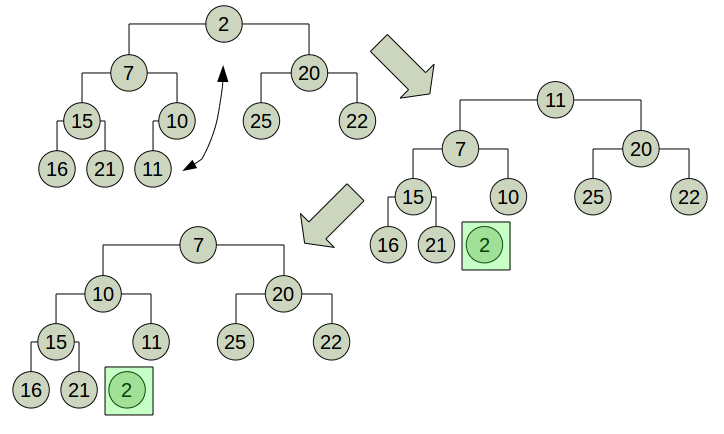
\includegraphics[height=9cm]{aufg1}
\caption{Durch das Umsortieren ergibt sich eine Reihenfolge von [7,10,20,15,11,25,22,16,21,2].}
\end{figure}

\subsection*{Aufgabe 2}
F�r jedes Blattelement gilt, dass es einen Vater hat, wobei $a_{1} \geq a_{2}$, w�rde man einen Ast aufw�rts nummerieren.\\
Schritt: Da auch der jeder Vater ein Unterelement eines Vaters $a_{3}$ ist, muss auch hier gelten $a_{2} \geq a_{3}$. Da dies unabh�ngig f�r jeden Ast gilt, muss f�r das Wurzelelement $a_{n}$, worin alle Teilb�ume zusammelaufen, gelten: $a_{1} \geq a_{2} \geq \cdots \geq a_{n}$. Somit muss die Wurzel den kleinsten vorkommenden Wert enthalten.

\subsection*{Aufgabe 3}
Ein absteigend sortiertes Feld ist ein Max-Heap (sofern darin keine doppelten Elemente vorkommen), weil f�r jedes Element $a_{n}$ gilt, dass $a_{n} > a_{n+1} > a_{n+2}$. Dies enstpricht der Max-Heap-Bedingung: Da auch auf tieferen Stufen des Baumes dieses Prinzip gelten muss, muss auch $a_{n} > a_{n+t1} > a_{n+t2}$ gelten, wobei $t1, t2 \geq 1$.

\subsection*{Aufgabe 4}
\begin{figure}[ht]
\centering
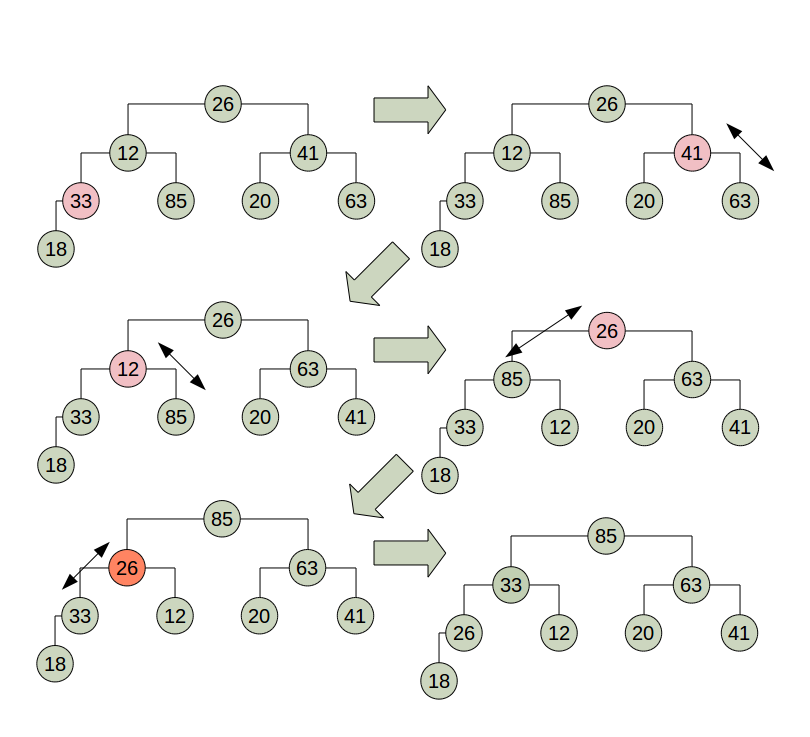
\includegraphics[height=9cm]{aufg4}
\caption{Die Blattelemente ausgeschlossen wird von unten her jedes Element durchgegangen und \texttt{MAX-HEAPIFY} ausgef�hrt. Erst bei der 5. Abbildung muss jedoch zwecks Verletzung der Heap-Eigenschaft auf die unteren Knoten zugegriffen werden.}
\end{figure}

\clearpage
\subsection*{Aufgabe 5}
$T(n)$ von Heap sort in den beiden F�llen, wenn das Feld schon absteigend bzw. aufsteigend sortiert ist:
\begin{itemize}
 \item Bei einem Max-Heap, welcher absteigend sortiert ist, ist die Laufzeit minimal. Dies f�hrt zu folgender Annahme: $O(n)$ wird ben�tigt, um den Heap zu konstruieren. F�r das Absenken der Elemente wird jedoch nur eine konstante Zeit verwendet, da jedes Element schon am richtigen Ort ist: $\Theta(1)$. Zusammengez�hlt ergibt $\Theta(1) * \Theta(n) = \Theta(n)$.
 \item Bei einem Max-Heap, der initial aufsteigend sortiert ist, also der \textit{Worst Case}, muss jeder der B�ume beachtet werden. Wenn jedes Element abgesenkt werden muss, f�hrt dies zu einer Laufzeit von $\Theta(n) * \Theta(log_{2} n) = \Theta(n \cdot log n)$
\end{itemize}

\subsection*{Aufgabe 6}

\begin{figure}[ht]
\begin{minipage}[b]{0.45\linewidth}
\centering
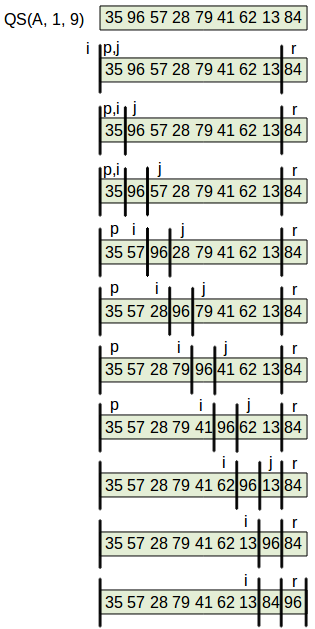
\includegraphics[height=8cm]{aufg6}
\caption{Beim ersten Aufruf wird die Zahl 96 heraufgesiebt und anscheinend mit dem pivot 84 getauscht.}
\end{minipage}
\hspace{0.5cm}
\begin{minipage}[b]{0.45\linewidth}
\centering
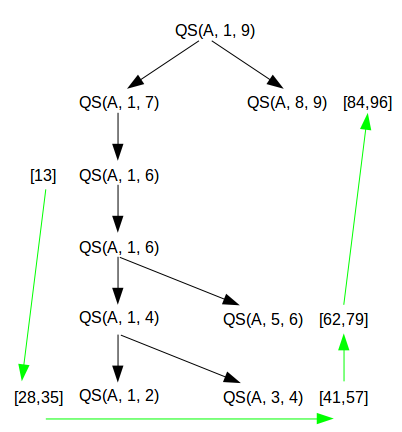
\includegraphics[height=8cm]{aufg6_2}
\caption{Die obenstehenden Aufrufe von Quicksort m�ssen gemacht werden, damit das Feld vollst�ndig sortiert ist.}
\end{minipage}
\end{figure}

\section*{Praktische Aufgaben}
\subsection*{Aufgabe 1}
Siehe \texttt{NameVornameComparator.java} und den entsprechenden Output \texttt{MiniTestApp.out}.

\subsection*{Aufgabe 2}
\begin{figure}[ht]
\centering
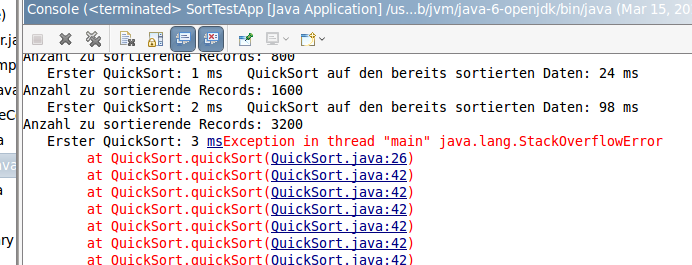
\includegraphics[height=4cm]{aufg_p2}
\caption{Ausgabe von \texttt{SortTestApp.java}.}
\label{pic:aufg_p2}
\end{figure}
Wie auf Abbildung \ref{pic:aufg_p2} angezeigt, wird ein \textit{Stack Overflow Error} ausgel�st. Dies ist wahrscheinlich der Fall, weil Quicksort sich selbst rekursiv zu viele Male aufgerufen hat; Die daraus entstehende Kette von noch zu verarbeitenden Funktionsaufrufen wurde zu lang, als dass die Java VM diese noch verarbeiten k�nnte. Dies ist auch der Grund, weshalb der zweite Durchlauf mit sortiertem Input massiv l�nger braucht (Faktor 50 bei 1600 Elementen).\\
Eine so grosse Anzahl von Selbstaufrufen ist der Fall, weil eine bereits sortierte Menge nochmals sortiert werden sollte. Hierbei wird jedoch immer nur das letzte Element abgetrennt (der Pivot) und der Rest mit einem erneuten Aufruf von Quicksort zu sortieren versucht. Dies wiederholt sich beim \textit{Stack Overflow Error} so lange, bis die Anzahl Aufrufe zuviel werden; Bei gr�sser werdenden $n$ braucht es auch $n$ Aufrufe von Quicksort.

\subsection*{Aufgabe 3}
Siehe \texttt{Quicksort.java} und den entsprechenden Output \texttt{Quicksort.out}.
\end{document}
